\subsection*{Grain and key}

One Silver row is one stop of one trip on one service date, with the key
\code{journey\_id + service\_date + stop\_order}. That is the smallest unit where punctuality
makes sense, and it keeps Silver useful for other questions than ours. \code{service\_date}
comes from \code{DataFrameRef} in the feed, not from the clock, so a trip at 00:30 belongs to
the right operating day. Silver also computes the arrival and departure delay in seconds
(actual or expected minus aimed) and keeps \code{snapshot\_time}, \code{run\_id} and
\code{call\_status} (recorded or estimated).

\subsection*{Parsing}

We tried Spark's XML reader first. It dropped the \code{+01:00} from the timestamps, which
would have shifted every delay by an hour without any error, and it gave recorded and
estimated stops different structures. So we parse each file with Python's ElementTree inside
Spark tasks and convert all times to UTC:

\begin{lstlisting}
# 20:00 the day before to 02:59 the day after
paths = list_bronze_files(root, start, end)
# one task per file, so a task only holds one snapshot in memory
results = sc.parallelize(paths, len(paths)).map(read_file) \
            .persist(StorageLevel.MEMORY_AND_DISK)
\end{lstlisting}

One task per file comes from our first prod run, which ran out of memory: Spark had put 288
files into 4 big tasks. Bronze folders are UTC days, while a night bus of day $D$ can show up
in the files of the next day, so Silver reads from 20:00 the evening before to 02:59 the
morning after, and only writes day $D$ (Section~\ref{sec:perf}).

\subsection*{Reject or flag}

A rejected row is gone for the analysis, while a flagged row can still be used or left out
later. So we only reject rows that can never give a delay and flag the rest
(Table~\ref{tab:rules}). Rejected rows are saved in \code{silver/rejected\_calls} with the code
of the first rule they fail. The rules run before deduplication, so a broken row can never be
the copy that is kept. In 27 days no row was rejected.

\begin{table}[htb]
\caption{Silver rules. Cancelled trips stay in Silver so Gold can count cancellations.}
\label{tab:rules}
\centering\small
\renewcommand{\arraystretch}{1.2}
\begin{tabularx}{\linewidth}{@{}ll>{\raggedright\arraybackslash}X@{}}
\toprule
& Rule & Why \\
\midrule
Reject & \code{MISSING\_KEY} & no journey, service date or stop order, so no deduplication \\
Reject & \code{MISSING\_LINE\_OR\_STOP} & cannot be grouped in Gold \\
Reject & \code{MISSING\_AIMED\_TIME} & no aimed time, so no delay \\ \rowline
Flag & \code{is\_missing\_actual} & no actual or expected time \\
Flag & \code{is\_delay\_outlier} & delay below $-10$\,min or above 3\,h \\
Flag & \code{is\_bad\_stop\_name} & name contains \code{Ã} (UTF-8 read as Latin-1) \\
Flag & \code{exclude\_from\_punctuality} & cancelled, outlier or no actual time \\
\bottomrule
\end{tabularx}
\end{table}

The outlier limits were a guess at first. We checked them on 11 days of prod data: 99.8\% of
stops are between $-5$ and $+60$ minutes, with a median of $+2.2$. The 702 stops below
$-10$ minutes were mostly times from the day before, and the 17 above 3 hours came from two
trips shifted by 4 to 11 hours on every stop. These are feed errors, so we kept the limits.

\subsection*{Removing duplicates}

Every stop is repeated in about 22 snapshots. On 2 November the snapshots had 3{,}401{,}155
stop rows, which became 153{,}568 stops. \code{dropDuplicates} would keep a random copy, but
we want the best one, so we use a window:

\begin{lstlisting}
w = Window.partitionBy("journey_id", "service_date",
                       "stop_order").orderBy(
    # real time before prediction
    (F.col("call_status") == "recorded").desc(),
    # then the newest snapshot
    F.col("snapshot_time").desc(),
    # same snapshot twice: stable choice
    F.col("run_id").desc())
df.withColumn("_rn", F.row_number().over(w)) \
  .filter("_rn = 1").drop("_rn")
\end{lstlisting}

We added \code{run\_id} after the double fetch on 27 October: two copies of the same snapshot
had the same \code{snapshot\_time}, Spark picked one at random, and two reruns of the same day
did not give the same result.

\subsection*{Quality table and reruns}

Every run appends its numbers to \code{silver/quality}, one row per metric (23 per run): rows
read, unparseable rows, rejected rows per reason, nulls, each flag, duplicates before and
after deduplication, a schema check, and files read and skipped. With one row per metric we can
add metrics without changing the table. Figure~\ref{fig:funnel} follows one day through
Silver, and Figure~\ref{fig:quality} shows the Silver rows and flags for every service day.

\begin{figure}[!htbp]
\centering
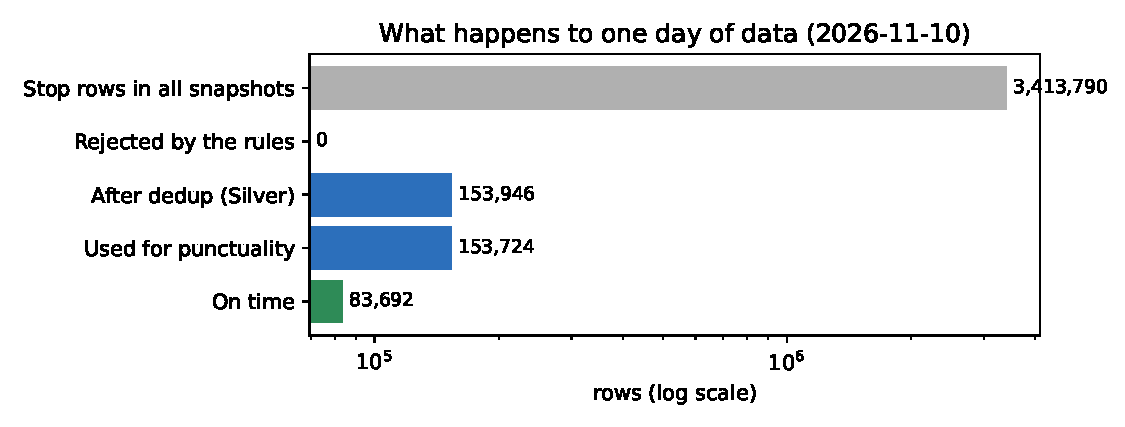
\includegraphics[width=0.85\linewidth]{3_silver_funnel.pdf}
\caption{One day through Silver, from the rows read to the rows written.}
\label{fig:funnel}
\end{figure}

\begin{figure*}[t]
\centering
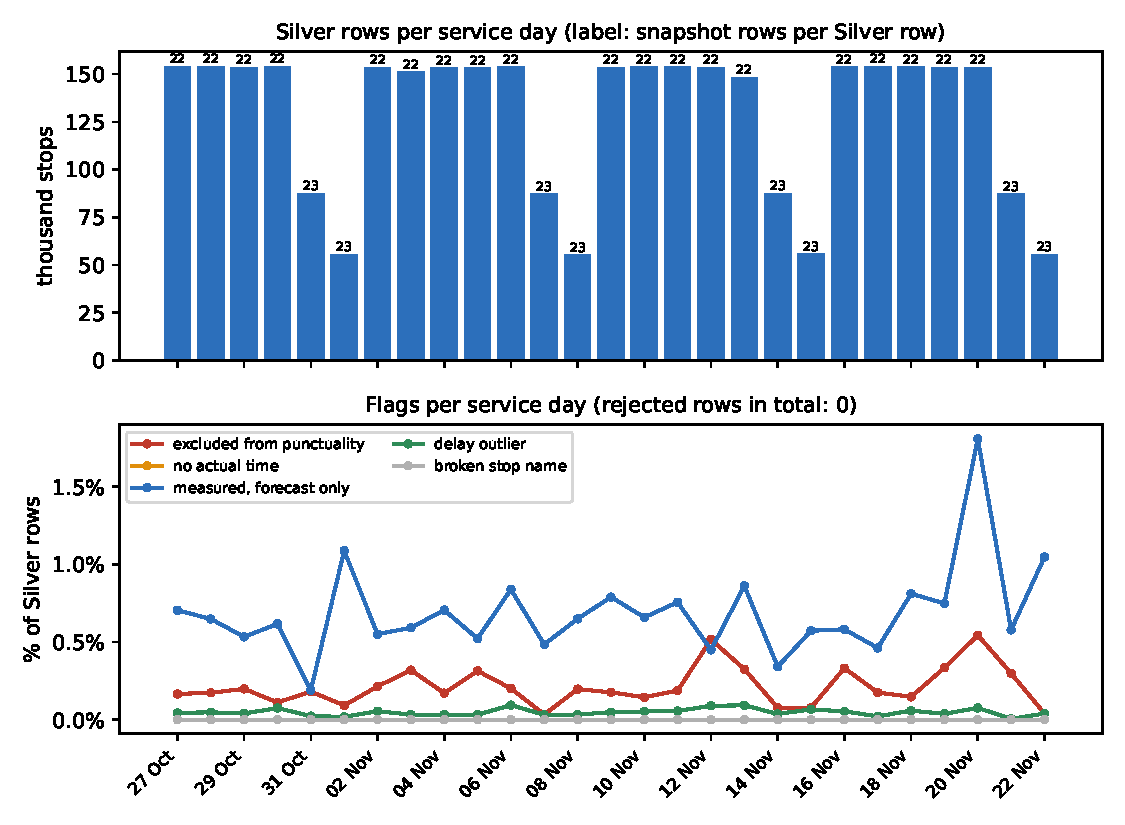
\includegraphics[width=0.85\textwidth]{7_quality_per_day.pdf}
\caption{Silver rows and flags per service day, from the quality table.}
\label{fig:quality}
\end{figure*}

A Bronze file that cannot be read is skipped and counted. If more than 5\% of the files fail,
Silver stops before writing anything: at that point a bug in our code is more likely than bad
data, and we do not want a good day replaced by a partial one. Silver is written as Parquet
partitioned by \code{service\_date} with dynamic partition overwrite, so a rerun only replaces
the days it builds.
